\part{Les données}
    \chapter{Le périmètre produit}
    \label{perimetre_produit}
        \section{Accessibilité de la donnée en fonction des branches}

        Comme vu à la section \ref{outils_infos} page \pageref{outils_infos}, les systèmes d'information associés à la gestion de l'information produit offrent des niveaux d'accès hétérogènes à la donnée produit.
        Le récapitulatif par branche est le suivant : 
        \begin{description}
            \item[\'{E}piSaveurs :] on peut simplement accéder à l'ensemble des données produit, structurées, non structurées (i.e. textes longs) et pièces jointes
            \item[PassionFroid :] on a uniquement la possibilité d'exporter manuellement les données structurées articles depuis le système de gestion SAP.
            Elles permettent de produire quelques analyses quantitatives.
            Il est difficile de faire des exports en masse de l'outil de gestion de l'information produit GIP (cf. section \ref{GIP} page \pageref{GIP}).
            \item[TerreAzur :] idem PassionFroid, si ce n'est qu'en plus le système GIP n'est pas utilisé au sein de cette branche.
            \item[Délice et Création :] le système d'information ne permet pas d'exporter les données et donc de produire des indicateurs détaillés. On peut toutefois avoir des informations quantitatives de la part des opérationnels.
            \item[Saveurs d'Antoine :] idem Délice et Création
            \item[Pomona Suisse :] la branche est en cours de structuration, et les référentiels articles ne sont pas partagés entre les succursales. Il n'est pas possible d'obtenir d'information quantitative sur ces données.
            \item[Pomona Iberia :] idem Pomona Suisse
        \end{description}

        \section{Analyses quantitatives}
            \subsection{Comparatifs entre les branches}

                Les graphes de cette section ont été produits via le code présenté en annexe, au chapitre \ref{code:analyse_quantitative} page \pageref{code:analyse_quantitative}


                \begin{figure}[htbp]
                    \begin{center}
                    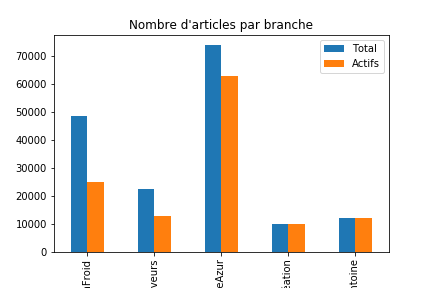
\includegraphics[width=\linewidth]{img/Articles par branche.png}
                    \end{center}
                    \caption{Volumétrie article par branche}
                    \label{fig:volumetrie_article}
                \end{figure}          

                histogramme avec pour chaque branche le nombre d'article et de produits

                +variante en retirant les statuts inactifs

            \subsection{Les types de produits}

            Focus sur les branches Jupiter.
            Par type d'article / groupe de marchandises / groupe d'article, en retirant les articles inactifs. Toujours avec la vision article et produit (FIA).

            Ajout aussi du niveau 1 de la hiérarchie produit. Voir la possibilité de faire une représentation en 2D (type art / hiérarchie)

    \chapter{Les données utilisables}
        \large
        Comme vu au chapitre \ref{perimetre_produit} page \pageref{perimetre_produit}, les données produit ne sont simplement accessibles que pour la branche \'{E}piSaveurs.
        On se focalisera donc sur cette branche pour la suite de cette étude.
        \normalsize

        \section{Données structurées}

        Les données dites structurées sont l'ensemble des données qui peuvent prendre leurs valeurs dans un domaine restreint.
        Par exemple, ce sont les données booléennes, les choix issus de listes déroulantes, les valeurs numériques\dots
        Les principales données structurées pour les produits alimentaires dans le PIM sont : 
        \begin{description}
            \item[le code du produit :] calculé par le système
            \item[le fournisseur :] référence croisée vers le code du fournisseur
            \item[le type de produit :] épicerie, boisson alcoolisée, hygiène, chimie, boisson non-alcoolisée
            \item[le type d'unité de base :] paquet, boîte, sachet, rouleau, bouteille, pot, \dots
            \item[le GTIN du produit :] identifiant numérique unique, utilisé entre autres pour l'étiquetage sous forme de code à barres\cite{GS1_GTIN}
            \item[les poids :] brut, net, net égoutté (pour les conserves)
            \item[le volume :] pour les produits liquides
            \item[les durées de vie :] le type (Date Limite de Consommation ou Date de Durabilité Minimale) et la durée (totale à fin de production, garantie à livraison)
            \item[les modes de conservation avant/après ouverture :] à température ambiante, au réfrigérateur puis à consommer sous 2 jours, \dots
            \item[les labels :] le(s) label(s) s'appliquant au produit (cf. section \ref{labels} page \pageref{labels})
            \item[les régimes particuliers :] Halal, Casher, Sans porc, Végétarien, Végétalien, \dots
            \item[les caractéristiques spéciales :] sans OGM, non traité par ionisation
            \item[la présence d'allergènes :] le niveau de présence de chacun des 14 allergènes réglementés (cf. section \ref{composition} page \pageref{composition})
            \item[les matières grasses utilisées :] palme, beurre, coco, tournesol, palmiste, \dots
            \item[les additifs présents :] les codes Exxx et les fonctions des additifs mis en oeuvre \cite{additifs_regl_eu}\cite{additifs_wiki}
            \item[les données nutritionnelles obligatoires :] pour 100g ou 100mL, valeur énergétique (en kJ et kcal), matières grasses, dont acides gras saturés, Glucides, dont sucres simples, Fibres, Protéines, simplement
            \item[les données nutritionnelles facultatives :] vitamines, minéraux, omégas, \dots
            \item[les allégations nutritionnelles :] riche en, faible en, sans,\dots associé à un nutriment défini dans les 2 points précédents
            \item[le nutriscore :] note allant de A à E, définie dans la loi Santé de janvier 2016
            \item[le taux de TVA :] un des quatre taux définis dans la réglementation française
            \item[le code nomenclature douanière :] code identifiant les marchandises défini par les douanes pour la Déclaration d'\'{E}change de Biens\cite{notions_DEB}
            \item[le pays d'origine pour la DEB :] le pays d'origine à déclarer dans la Déclaration d'\'{E}change de Biens\cite{notions_DEB}
            \item[] 
        \end{description}
        
        
        \section{Données non structurées}
        
        Les listes d'ingrédients juste une liste ordonnées d'ingrédients triés par ordre décroissant de quantité mise en oeuvre.

        Parfois détaillé par phase, mais en général déconseillé.
        \section{Pièces jointes}
            \label{pieces_jointes}

            Dans chacune des sections, mentionner la volumétrie de données accessibles (avec les facettes migration, statuts, \& compagnie) et tout

            \subsection{Fiches techniques fournisseur}
            \subsection{\'{E}tiquettes produit}
            \subsection{Fiches logistiques fournisseur}
            \subsection{Fiches techniques et argumentaires Pomona}
        \section{Récapitulatif de la complétude des données}

        Mettre ici un ou plusieurs tableaux récapitulatifs illustrant les données possédées quantitativement.

        \section{Analyse qualitative des données}
        
        Montrer qu'un sondage basique fait que la qualité actuelle est perfectible

        Mettre également la distribution numérique des produits par fournisseur et insister sur la difficulté posée par de multiples formats

        Dire ici qu'il y a finalement beaucoup de pdf qui possèdent des textes extractibles vs. uniquement des images.

        \section{Les données \og manuellement étiquetées \fg}

        Montrer comment elles ont été produites

        Expliciter les règles de gestion qui ont été listées pendant l'étiquetage manuel

        Evaluer la cohérence entre étiquettes manuelles et contenu du PIM
